\documentclass[10pt,a4paper]{article}

% Language setting
\usepackage[british]{babel}

% Set page size and margins
\usepackage[a4paper,top=2cm,bottom=2cm,left=2.5cm,right=2.5cm,marginparwidth=1.75cm]{geometry}

\usepackage[style=ieee, backend=biber]{biblatex} % IEEE style citations using biblatex
\addbibresource{references.bib} % Your .bib file


\usepackage{amsmath}
\usepackage{graphicx}
\usepackage[colorlinks=true, allcolors=blue]{hyperref}
\usepackage{hyperref}
\usepackage{orcidlink}
\usepackage[title]{appendix}
\usepackage{mathrsfs}
\usepackage{amsfonts}
\usepackage{booktabs} % For \toprule, \midrule, \botrule
\usepackage{caption}  % For \caption
\usepackage{threeparttable} % For table footnotes
\usepackage{algorithm}
\usepackage{algorithmicx}
\usepackage{algpseudocode}
\usepackage{listings}
\usepackage{enumitem}
\usepackage{chngcntr}
\usepackage{booktabs}
\usepackage{lipsum}
\usepackage{subcaption}
\usepackage{authblk}
\usepackage[T1]{fontenc}    % Font encoding
\usepackage{csquotes}       % Include csquotes
\usepackage{diagbox}


% Customize line spacing
\usepackage{setspace}
\onehalfspacing % 1.5 line spacing

% Redefine section and subsection numbering format
\usepackage{titlesec}
\titleformat{\section} % Redefine section numbering format
  {\normalfont\Large\bfseries}{\thesection.}{1em}{}
  
% Customize line numbering format to right-align line numbers
\usepackage{lineno} % Add the lineno package
\renewcommand\linenumberfont{\normalfont\scriptsize\sffamily\color{blue}}
\rightlinenumbers % Right-align line numbers

\linenumbers % Enable line numbering

% Change the position of the table caption above the table
\usepackage{float}   % for customizing caption position
\usepackage{caption} % for customizing caption format
\captionsetup[table]{position=top} % caption position for tables

% Define the unnumbered list
\makeatletter
\newenvironment{unlist}{%
  \begin{list}{}{%
    \setlength{\labelwidth}{0pt}%
    \setlength{\labelsep}{0pt}%
    \setlength{\leftmargin}{2em}%
    \setlength{\itemindent}{-2em}%
    \setlength{\topsep}{\medskipamount}%
    \setlength{\itemsep}{3pt}%
  }%
}{%
  \end{list}%
}
\makeatother

% Suppress the warning about \@parboxrestore
\pdfsuppresswarningpagegroup=1


%-------------------------------------------
% Paper Head
%-------------------------------------------
\title{[Paper title]}

\author{
    First Last name (\texttt{OsirisID}), 
    First Last name (\texttt{OsirisID})
}

\date{}  % Remove date

\begin{document}
\maketitle

\textbf{Overall comment:}
A paper needs to introduce your study and state why it is relevant. It should clearly explain how you performed the study, its analyses and all its components and why you did so. Based on the methodology section, other researchers need to be able to replicate your results. Subsequently, results are reported in an unbiased and scientifically acceptable way such that readers can easily understand the important aspects of your results. Finally, the paper should discuss the impact of its results by comparing to other work and reflecting on it and drive the point home in a conclusion. At all times, the paper should be grounded and well justified using literature, empirical evidence, or solid reasoning.

This video explains how to write a good paper in a very enjoyable and easy-to-understand presentation: \url{https://www.youtube.com/watch?v=VEXaUHNmpQw}. I also like this webpage from Paul Graham explaining why a simple text is a better text: \url{https://paulgraham.com/simply.html}. 

\textbf{Key points:}
\begin{itemize}
    \item Max. 12 pages excluding figures, tables, and references
    \item Adhere to the template as shown here
    \item \textbf{Keep sentences short and concise}
    \item Explain/justify all choices via a reference, formal proof, empirical proof, or solid reasoning
    \item Use IEEE citation style
\end{itemize}

%-------------------------------------------
% Paper Body
%-------------------------------------------
\section{Introduction}\label{sec:introduction}
The introduction is your chance to grab the reader's attention and set the stage for your research. It should spark interest and provide enough context for the audience to understand the text ahead. In addition to informing the reader, it should also explain your work's impact on science and society and why your study is worth reading. TIP: Think about the issue you are trying to solve and why that is so important.

Begin by introducing a broad issue that resonates with your target audience. For example, if you are researching the impact of social media on mental health in teenagers, you could start with a statistic about overall social media usage among teens. Gradually narrow your focus by highlighting a specific issue, such as the potential link between increased social media use and anxiety symptoms. Emphasize why this is an issue that needs to be solved and describe how you intend to do this. However, do not reveal details about the study and its results yet! 

Throughout your introduction, use relevant, credible, and up-to-date references to support your claims. This demonstrates your understanding of the field and strengthens the foundation of your research.

In contrast to the research proposal, your research question should already become clear when reading the introduction. You do not have a section specifically dedicated to the research question. You should introduce it in the introduction instead. Note, this is often NOT in a literal way (i.e., using quotation marks around your research question). Instead, try to introduce it in the flow of your introduction. Nevertheless, some papers include a short list of bullet points explaining the contributions of their work at the end of their introduction. 

All introductions end by giving a short overview of what is to come. Talk about your upcoming sections and what they describe. This signals the end of the introduction.

\section{Related work}\label{sec:relatedwork}
In most cases, you are not the first to study your topic in science. The related work section allows you to present and discuss previous works that relate to your idea. Note that this should not merely be a list of previous works and what they did. Try to distill, describe, and discuss overarching themes in methods and results. This section should be heavily cited. 

Often, there will not be many papers that pursue your exact idea and methodology. Hence, the related work section is often split up into different sections where each section focuses on a specific aspect of your proposed research idea. For example, when researching dementia diagnosis in elderly people using remote healthcare solutions, one section could summarize the works on dementia diagnosis, while another could focus on the use of wearables in the elderly patient population. These sections can start out from a very broad focus and gradually narrow down on your exact research questions. Remember that literature closer to your study is more important than studies further away. Hence, try to include more references to studies that are more relevant for your study than those that are less relevant.

As you discuss previous studies, do not shy away from critical analysis. However, make sure to support your criticism well. Highlight the strengths and limitations of existing research, and explain how your study aims to address any gaps in knowledge. 

\section{Methodology}\label{sec:methods}
In this section you describe what, why, and how you got the results of your study. Explain all steps of the analysis process, like feature extraction, statistical analysis, etc. Also, explain all the resources you used. In case you are using a dataset, describe all the necessary information of this dataset such that the reader does not have to read the other paper to understand yours. Yet, in all cases, refer to the original dataset's paper if the reader wants to know more. 

Describe and explain your methodology as detailed as possible. Often, papers use diagrams, equations, or pseudocode to explain their idea and methods as clearly and as unambiguously as possible. Place yourself in the reader's shoes and be very critical about what you read and, more importantly, what you do not read. Your explanations should be clear and comprehensive enough for someone else to replicate your study. 

Be sure to justify your choices at each step. Explain why you have selected a specific data source, experimental design, or analytical technique. Connect these choices back to your research question and the type of data you will be working with.

The methods section does not have to sell your study anymore. Instead, it should be a very 'dry' and factual piece of text that describes all the steps involved and also why those steps were the best steps to take. Again, use solid reasoning or references to justify your decisions.

\subsection{Data}
Name the dataset you will use and its origin. Describe its contents, focus, the type of data, etc. As I said earlier, explain all the details a reader would need to understand your paper without reading the dataset's paper. Your paper should be understandable 'standalone'. Yet, do refer readers to the dataset's paper if they want to know more. Also, explain why this dataset is relevant to your research. 

\subsection{Preprocessing and feature extraction}
Specify which variables/features you analyzed and used and justify these choices. Describe how you extracted these features from your data. Describe the entire preprocessing and feature extraction pipeline as detailed as possible. Place yourselves in the reader's shoes and be critical about what you read and do not read. Identifying those holes in information is very hard. Do not shy away from asking friends, other classmates, or your parents to help you identify these gaps. It is very easy to forget details but it is very hard to provide too many details. If in doubt, describe it! Also, please feel free to use diagrams, equations, tables and/or pseudocode, to enrich your story. 

Side information: Nowadays, journals often ask for a main paper and a document containing supplementary information. The latter does not have a page limit and can sometimes grow up to 100 pages. This is how journals solve the issue of not having enough pages to spare to explain all the methodology's details while providing enough information for researchers to replicate results. If you feel like you do not have enough pages to include are your details, feel free to send me a supplementary information document as well. Yet, please do not send in 100-page documents. I still deem my sleep to be important as well :)

\subsection{Statistical analysis}
Describe and justify the specific statistical test(s) you will use to answer your research question. Begin by describing the large omnibus test that involves as many IV's and DV's as possible. Ideally, this omnibus test includes all of them. However, if you can provide solid reasoning and/or references to other works that show that the DV's are independent, you can analyse them separately using one test per DV. Justify all choices based on your research question and type of data and analysis. Describe your dependent and independent variables. 

A very important step of doing a statistical analyses is to check whether the assumptions of the test hold. For example, if using an ANOVA, check whether your data within each group is normally distributed, if your samples are independent and if you have homogeneity of variances. Use appropriate tests or solid reasoning to test/validate these assumptions. \textbf{This is an important part of your project!}

Next, describe the post-hoc analyses you will perform depending on the omnibus test to get a deeper understanding of the relationships between your IV's and DV's. This can be separate ANOVA's or pairwise t-tests if you performed a MANOVA as your omnibus test. Other options are regression analyses or even machine learning type analyses in which you try to predict the outcome of a DV based on the input of your IV's. In that case, split the data in a train and test dataset to prevent overfitting. 

I can imagine you still want to change or adapt your post-hoc analyses throughout the second phase based on new insights you gain from the lectures. You are free to do so and you can always contact me if you have questions about this.

\textbf{Note:}
\begin{itemize}
    \item Statistical analysis should include >1 independent and (>1 dependent variable or a within subjects design (both are also fine)). 
    \item Check whether assumptions underlying the selected statistical analysis are met. If not, provide a remedy or alternative analysis
    \item Report on post-hoc analysis or supplementary analysis including an appropriate type of regression analysis or a well-justified alternative
\end{itemize}

\section{Results}
The result section of your paper has the responsibility to inform the reader about your results as efficiently and unbiased as possible. You should choose the right type of visualization to highlight the most important parts of the results while also being honest and unbiased. Sometimes this is a difficult balance to strike. For example, when showing excerpts of your data, do not cherry pick those that support your findings but show a representative sample. Also, use boxplots and distribution plots whenever you can. Nowadays, it is seen as bad practice to only show the mean of your data (e.g., barplots representing the mean of each group). Instead, use boxplots or violin plots to inform the reader about the actual distribution within each group instead of an aggregated metric only.  

A figure can convey more than a thousand words. This is especially true for research papers. A well designed figure can make or break your results. Try to think about the best visualization for you study. Figures should always adhere to acceptable scientific standards meaning the figures should have a title, both axes should have labels and units assigned to them and all text should be readable when printed. 

A result section does NOT talk about the results. It only shows the results and provides the information needed to understand the results. It also does not provide any new information about the methodology as this should already have been provided in the methodology section. 

A result section does inform the reader about the outcome of the assumption checks and the results of the main omnibus test and the post-hoc analyses. Hence, it can reason about these results and explain which post-hoc tests were done based on intermediate results. However, all the tests described in this section should already have been introduced in the methodology section. 

\section{Discussion and conclusion}
The discussion section is often seen, together with the introduction, as the most important part of your paper. In this section, you connect your results back to your hypothesis, the related work, and its relevance as stated in your introduction. This is the place where you can reason about your results, talk about all the expected and unexpected results, and explain why these results are valid or not. This is also the place to talk about validity, limitations, and future work. Ground your discussion in the scientific field by using references to other works. Compare to existing works and explain why you got different results or why your results may confirm the findings of others. 

Often, the conclusion is merged with the discussion as the conclusion is generally only a single paragraph. As such, in this merged form, the conclusion is the last paragraph of this section. In this paragraph, you circle back to the issue and relevance stated in your introduction. You re-emphasize why your study was important, why the results are important and what future work could improve on. Try to close the circle and make the story whole.

% Print bibliography
\printbibliography

\newpage
\begin{appendices}

%--- Section ---%
\section{How to Include Equations}\label{sec4}

Equations in \LaTeX{} can either be inline or set as display equations. For
inline equations use the \verb+$...$+ commands. Eg: the equation
$H\psi = E \psi$ is written via the command \verb+$H \psi = E \psi$+.

For display equations (with auto generated equation numbers)
one can use the equation or eqnarray environments:
\begin{equation}
\|\tilde{X}(k)\|^2 \leq\frac{\sum\limits_{i=1}^{p}\left\|\tilde{Y}_i(k)\right\|^2+\sum\limits_{j=1}^{q}\left\|\tilde{Z}_j(k)\right\|^2 }{p+q},
\label{eq1}
\end{equation}
where
\begin{align}
D_\mu &=  \partial_\mu - ig \frac{\lambda^a}{2} A^a_\mu \nonumber \\
F^a_{\mu\nu} &= \partial_\mu A^a_\nu - \partial_\nu A^a_\mu + g f^{abc} A^b_\mu A^a_\nu
\label{eq2}
\end{align}
Notice the use of \verb+\nonumber+ in the align environment at the end
of each line, except the last, so as not to produce equation numbers on
lines where no equation numbers are required. The \verb+\label{}+ command
should only be used at the last line of an align environment where
\verb+\nonumber+ is not used.
\begin{equation}
Y_\infty = \left( \frac{m}{\textrm{GeV}} \right)^{-3}
    \left[ 1 + \frac{3 \ln(m/\textrm{GeV})}{15}
    + \frac{\ln(c_2/5)}{15} \right]
\label{eq3}
\end{equation}
The class file also supports the use of \verb+\mathbb{}+, \verb+\mathscr{}+ and
\verb+\mathcal{}+ commands. As such \verb+\mathbb{R}+, \verb+\mathscr{R}+
and \verb+\mathcal{R}+ produces $\mathbb{R}$, $\mathscr{R}$ and $\mathcal{R}$
respectively 
%(refer Subsubsection~\ref{subsubsec3}).

Equations must be provided as editable text, either in a Word or LaTeX source file. They should be numbered consecutively through the manuscript as shown in Equations \ref{eq1}, \ref{eq2} and \ref{eq3}. In APA style, when discussing numbered equations in the text, write out the word “Equation” and give the number. For example, you would write “see Equation \ref{eq1}.”
Use no punctuation after the equation if it appears at the end of a sentence; however, it is permissible (and may even be necessary) to place some form of punctuation after it (a comma or semi-colon, for example) if it appears in the middle of the sentence and is followed by text. In any case, maintain the coherence of all sentences with equations in them.


%--- Section ---%
\section{Tables}\label{sec5}

Use the table and tabular environments for basic tables --- see Tables~\ref{tab1} and \ref{tab2}, for example. Table \ref{tab1} is an sample figure including table footnotes. For more information, please see this help article on \href{https://www.overleaf.com/learn/latex/tables}{tables}. The general table style should only include horizontal rules at the top, after the header row, and at the bottom of the table. Tablenotes can be used to note small details otherwise too minor to be put in the main text.

\begin{table}[!ht]
\caption{Sample table with footnotes\label{tab1}}
\begin{threeparttable}
\begin{tabular*}{\columnwidth}{@{\extracolsep\fill}llll@{\extracolsep\fill}}
\toprule
column 1 & column 2 & column 3 & column 4\\
\midrule
row 1 & data 1 & data 2 & data 3 \\
row 2 & data 4 & data 5\tnote{1} & data 6 \\
row 3 & data 7 & data 8 & data 9\tnote{2} \\
\bottomrule
\end{tabular*}
\begin{tablenotes}
\item Source: This is an example of table footnote. This is an example of table footnote. This is an example of table footnote. This is an example of table footnote. This is an example of table footnote.
\item[1] Example for a first table footnote.
\item[2] Example for a second table footnote.
\end{tablenotes}
\end{threeparttable}
\end{table}

\begin{table*}[!ht]
\caption{Example of a lengthy table which is set to full textwidth.\label{tab2}}
\tabcolsep=0pt
\begin{threeparttable}
\begin{tabular*}{\textwidth}{@{\extracolsep{\fill}}lcccccc@{\extracolsep{\fill}}}
\toprule
& \multicolumn{3}{c}{Element 1\tnote{1}} & \multicolumn{3}{c}{Element 2\tnote{2}} \\
\cmidrule(lr){2-4}\cmidrule(lr){5-7}
Project & Energy & $\sigma_{\mathrm{calc}}$ & $\sigma_{\mathrm{expt}}$ & Energy & $\sigma_{\mathrm{calc}}$ & $\sigma_{\mathrm{expt}}$ \\
\midrule
Element 3 & 990 A & 1168 & $1547\pm12$ & 780 A & 1166 & $1239\pm100$ \\
Element 4 & 500 A & 961 & $922\pm10$ & 900 A & 1268 & $1092\pm40$ \\
\bottomrule
\end{tabular*}
\begin{tablenotes}
\item Note: This is an example of table footnote this is an example of table footnote this is an example of table footnote this is an example of~table footnote this is an example of table footnote.
\item[1] Example for a first table footnote.
\item[2] Example for a second table footnote.
\end{tablenotes}
\end{threeparttable}
\end{table*}


%--- Section ---%
\section{Figures}\label{sec6}

First you have to upload the image file from your computer using the upload link in the file-tree menu. Then use the includegraphics command to include it in your document. Use the figure environment and the caption command to add a number and a caption to your figure. See the code for Figure \ref{fig:frog} in this section for an example. As shown in Figures \ref{fig:frog} and \ref{fig:multi_figs}, the images should be single-page documents. 

Note that your figure will automatically be placed in the most appropriate place for it, given the surrounding text and taking into account other figures or tables that may be close by. You can find out more about adding images to your documents in this help article on \href{https://www.overleaf.com/learn/how-to/Including_images_on_Overleaf}{including images on Overleaf}.

\begin{figure}[!ht]
\centering
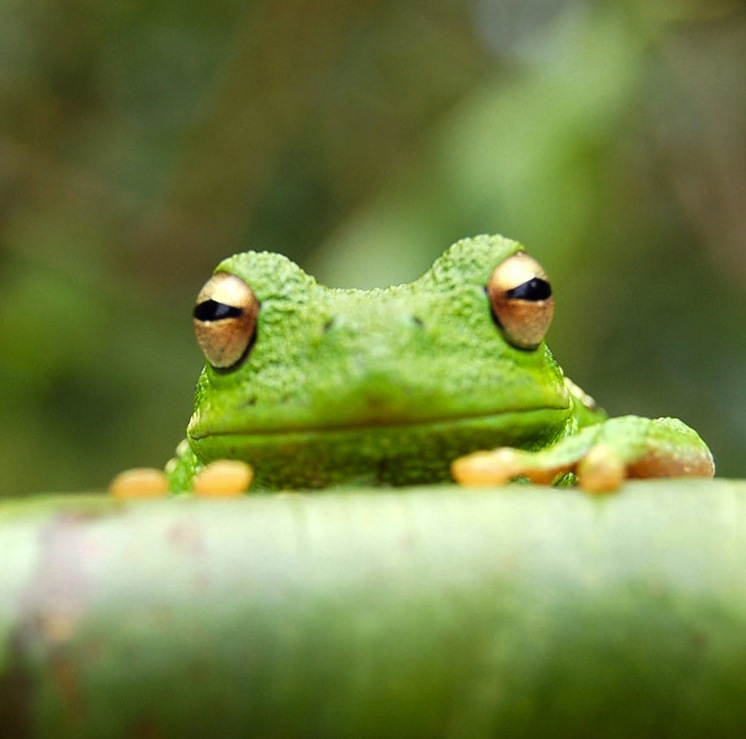
\includegraphics[width=0.4\linewidth]{figures/frog.jpg}
\caption{\label{fig:frog}This frog was uploaded via the file-tree menu.}
\end{figure}

\subsection{More information about figures}

As per display \LaTeX\ standards one has to use eps images for \verb+latex+ compilation and \verb+pdf/jpg/png+ images for
\verb+pdflatex+ compilation. This is one of the major differences between \verb+latex+
and \verb+pdflatex+. The images should be single-page documents. The command for inserting images
for \verb+latex+ and \verb+pdflatex+ can be generalized. The package used to insert images in \verb+latex/pdflatex+ is the
graphicx package. Figures can be inserted via the normal figure environment as shown in the below example:


\begin{figure}[!ht]
    \begin{subfigure}{0.3\textwidth}
        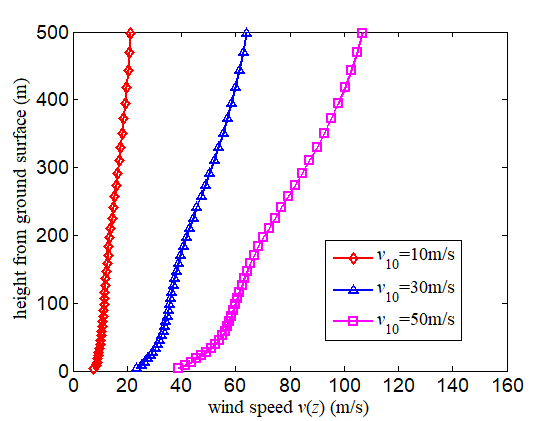
\includegraphics[width=\linewidth]{figures/fig_a.png}
        \caption{}
    \end{subfigure}
    \hfill
    \begin{subfigure}{0.3\textwidth}
        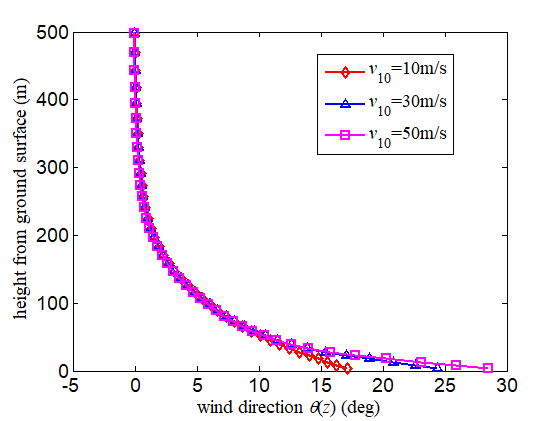
\includegraphics[width=\linewidth]{figures/fig_b.png}
        \caption{}
    \end{subfigure}
    \hfill
    \begin{subfigure}{0.3\textwidth}
        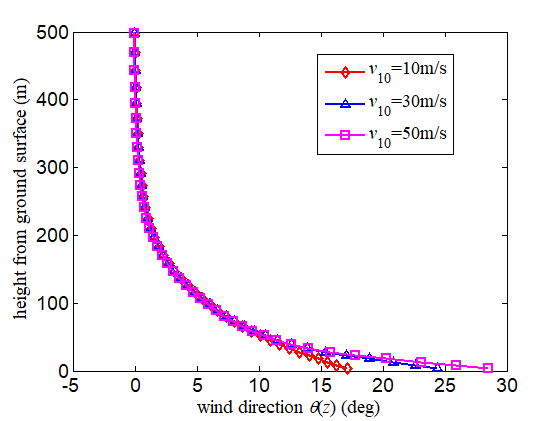
\includegraphics[width=\linewidth]{figures/fig_c.png}
        \caption{}
    \end{subfigure}
    \caption{Overall caption for the three figures: (a) caption for figure a, (b) caption for figure b, and (c) caption for figure c.}
    \label{fig:multi_figs}
\end{figure}


\begin{verbatim}
\begin{figure}[h]
        \centering\includegraphics{<eps-file>}
        \caption{<figure-caption>}
        \label{<figure-label>}
\end{figure}
\end{verbatim}


%--- Section ---%
\section{How to Include Algorithms, Program Codes, and Listings}\label{sec8}
Packages \verb+algorithm+, \verb+algorithmicx+, and \verb+algpseudocode+ are used for setting algorithms in latex.
For this, one has to use the below format:

\begin{verbatim}
\begin{algorithm}
\caption{<alg-caption>}\label{<alg-label>}
\begin{algorithmic}[1]
. . .
\end{algorithmic}
\end{algorithm}
\end{verbatim}

You may need to refer to the above-listed package documentation for more details before setting an \verb+algorithm+ environment.
To set program codes, one has to use the \verb+program+ package. We need to use the \verb+\begin{program}+ \verb+...+
\verb+\end{program}+ environment to set program codes.

\begin{algorithm}[!ht]
\caption{Calculate $y = x^n$}\label{algo1}
\begin{algorithmic}[1]
\Require $n \geq 0 \vee x \neq 0$
\Ensure $y = x^n$
\State $y \Leftarrow 1$
\If{$n < 0$}
        \State $X \Leftarrow 1 / x$
        \State $N \Leftarrow -n$
\Else
        \State $X \Leftarrow x$
        \State $N \Leftarrow n$
\EndIf
\While{$N \neq 0$}
        \If{$N$ is even}
            \State $X \Leftarrow X \times X$
            \State $N \Leftarrow N / 2$
        \Else[$N$ is odd]
            \State $y \Leftarrow y \times X$
            \State $N \Leftarrow N - 1$
        \EndIf
\EndWhile
\end{algorithmic}
\end{algorithm}

Similarly, for \verb+listings+, one has to use the \verb+listings+ package. To set environments similar to the \verb+verbatim+ environment, the \verb+\begin{lstlisting}+ \verb+... + \verb+\end{lstlisting}+ environment is used . Refer to the \verb+lstlisting+ package documentation for more details on this.

\begin{minipage}{\hsize}%
\lstset{language=Pascal}% Set your language (you can change the language for each code-block optionally)
\begin{lstlisting}[frame=single,framexleftmargin=-1pt,framexrightmargin=-17pt,framesep=12pt,linewidth=0.95\textwidth]
for i:=maxint to 0 do
begin
{ do nothing }
end;
Write('Case insensitive ');
Write('Pascal keywords.');
\end{lstlisting}
\end{minipage}


%--- Section ---%
\section{Lists}\label{sec7}

List in \LaTeX{} can be of three types: numbered, bulleted, and unnumbered. The ``enumerate'' environment produces a numbered list, the 
``itemize'' environment produces a bulleted list, and the ``unlist''
environment produces an unnumbered list.
In each environment, a new entry is added via the \verb+\item+ command.

\begin{enumerate}[label=\arabic*.]
\item This is the 1st item
\item Enumerate creates numbered lists, itemize creates bulleted lists, and unnumerate creates unnumbered lists.

\begin{enumerate}[label=\alph*.]
\item Second level numbered list. Enumerate creates numbered lists, itemize creates bulleted lists, and description creates unnumbered lists.
\item Second level numbered list. Enumerate creates numbered lists, itemize creates bulleted lists, and description creates unnumbered lists.

\begin{enumerate}[label=(\roman*)]
\item Third level numbered list. Enumerate creates numbered lists, itemize creates bulleted lists, and description creates unnumbered lists.
\item Third level numbered list. Enumerate creates numbered lists.
\end{enumerate}

\item Second level numbered list. Enumerate creates numbered lists, itemize creates bulleted lists, and description creates unnumbered lists.
\end{enumerate}

\item Numbered lists continue.
\end{enumerate}
Lists in \LaTeX{} can be of three types: enumerate, itemize, and description.
In each environment, a new entry is added via the \verb+\item+ command.

\begin{itemize}
\item First level bulleted list. This is the 1st item
\item First level bulleted list. Itemize creates bulleted lists, and description creates unnumbered lists.

\begin{itemize}
\item Second level dashed list. Itemize creates bulleted lists, and description creates unnumbered lists.
\item Second level dashed list. Itemize creates bulleted lists, and description creates unnumbered lists.
\end{itemize}

\item First level bulleted list. Bullet lists continue.
\end{itemize}

\noindent
Example for unnumbered list items:

\begin{unlist}
\item Sample unnumberd list text. Sample unnumberd list text. Sample unnumberd list text. Sample unnumberd list text. Sample unnumberd list text.

\item Sample unnumberd list text. Sample unnumberd list text. Sample unnumberd list text.

\item Sample unnumberd list text. Sample unnumberd list text. Sample unnumberd list text. Sample unnumberd list text. 
\end{unlist}


%--- Section ---%
\section{References}

You can simply upload a \verb|.bib| file containing your BibTeX entries or add bibtex code to the 'references.bib' file. You can then cite entries from it, like this: \cite{navarro2013learning}. We require you to use the \href{https://www.bath.ac.uk/publications/library-guides-to-citing-referencing/attachments/ieee-style-guide.pdf}{IEEE citation style}, which is already incorporated into this template. 

TIP: You can easily obtain a paper's bibtex code using Google Scholar.


\end{appendices}

\end{document}